\section{Casi d'uso}

\subsection{UC8 - Movimenti direzionali}
\begin{figure}[h!]\centering
    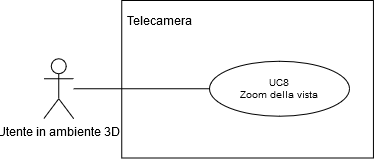
\includegraphics[scale=0.7]{template/images/UC8.png}
    \caption{UC8 - Movimenti direzionali}
\end{figure}
\begin{itemize}    
    \item \textbf{Attore:} utente;
    \item \textbf{Descrizione:} Compiere movimenti direzional significa che in ambiente di visualizzazione del grafico 3D l'utente, 
    tramite comandi opportuni, può interagire con il grafico compiendo degli spostamenti lungo i tre assi principali
    \item \textbf{Precondizioni:}    
        \begin{itemize}
            \item Il caricamento del dataset è avvenuto con successo.
            \item La generazione dell'ambiente 3D e del relativo grafico non hanno riscontrato errori.
            \item Vengono eseguiti i comandi opportuni per i vari spostamenti.
        \end{itemize}    
    \item \textbf{Postcondizioni:}
        \begin{itemize}
            \item La telecamera che inquadra il grafico nell'ambiente 3D si troverà in una posizione diversa da quella in cui si trovava prima di compiere lo spostamento.
        \end{itemize}    
    \item \textbf{Scenario:} 
        \begin{itemize}
            \item L'utente interagisce con l'ambiente 3D per compiere un movimento direzionale.
        \end{itemize}
\end{itemize}
\subsubsection{UC8.1 - Movimento direzionale asse X}
\begin{itemize}    
    \item \textbf{Attore:} utente;
    \item \textbf{Descrizione:} L'utente interagisce opportunamente con l'ambiente 3D per spostarsi in profondità.
    \item \textbf{Precondizioni:}    
        \begin{itemize}
            \item Il caricamento del dataset è avvenuto con successo.
            \item La generazione dell'ambiente 3D e del relativo grafico non hanno riscontrato errori.
            \item Vengono eseguiti i comandi opportuni per lo spostamento lungo l'asse X.
        \end{itemize}    
    \item \textbf{Postcondizioni:}
        \begin{itemize}
            \item La telecamera che inquadra il grafico nell'ambiente 3D si troverà in una posizione diversa da quella in cui si trovava prima di compiere lo spostamento rispetto all'asse X.
        \end{itemize}    
    \item \textbf{Scenario:} 
        \begin{itemize}
            \item L'utente interagisce con l'ambiente 3D per compiere un movimento direzionale lungo l'asse X.
        \end{itemize}
\end{itemize}
\subsubsection{UC8.2 - Movimento direzionale asse Y}
\begin{itemize}    
    \item \textbf{Attore:} utente;
    \item \textbf{Descrizione:} L'utente interagisce opportunamente con l'ambiente 3D per spostarsi in orizzontale.
    \item \textbf{Precondizioni:}    
        \begin{itemize}
            \item Il caricamento del dataset è avvenuto con successo.
            \item La generazione dell'ambiente 3D e del relativo grafico non hanno riscontrato errori.
            \item Vengono eseguiti i comandi opportuni per lo spostamento lungo l'asse Y.
        \end{itemize}    
    \item \textbf{Postcondizioni:}
        \begin{itemize}
            \item La telecamera che inquadra il grafico nell'ambiente 3D si troverà in una posizione diversa da quella in cui si trovava prima di compiere lo spostamento rispetto all'asse Y.
        \end{itemize}    
    \item \textbf{Scenario:} 
        \begin{itemize}
            \item L'utente interagisce con l'ambiente 3D per compiere un movimento direzionale lungo l'asse Y.
        \end{itemize}
\end{itemize}
\subsubsection{UC8.1 - Movimento direzionale asse Z}
\begin{itemize}    
    \item \textbf{Attore:} utente;
    \item \textbf{Descrizione:} L'utente interagisce opportunamente con l'ambiente 3D per spostarsi in verticale.
    \item \textbf{Precondizioni:}    
        \begin{itemize}
            \item Il caricamento del dataset è avvenuto con successo.
            \item La generazione dell'ambiente 3D e del relativo grafico non hanno riscontrato errori.
            \item Vengono eseguiti i comandi opportuni per lo spostamento lungo l'asse Z.
        \end{itemize}    
    \item \textbf{Postcondizioni:}
        \begin{itemize}
            \item La telecamera che inquadra il grafico nell'ambiente 3D si troverà in una posizione diversa da quella in cui si trovava prima di compiere lo spostamento rispetto all'asse Z.
        \end{itemize}    
    \item \textbf{Scenario:} 
        \begin{itemize}
            \item L'utente interagisce con l'ambiente 3D per compiere un movimento direzionale lungo l'asse Z.
        \end{itemize}
\end{itemize}

\subsection{UC9 - Riposizionamento iniziale}
\begin{figure}[h!]\centering
    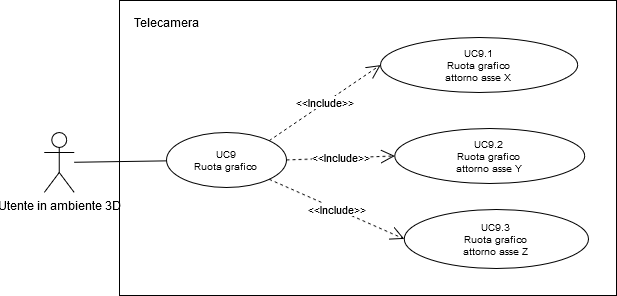
\includegraphics[scale=0.7]{template/images/UC9.png}
    \caption{UC9 - Riposizionamento iniziale}
\end{figure}
\begin{itemize}    
    \item \textbf{Attore:} utente;
    \item \textbf{Descrizione:} Effettuare un'azione di riposizionamento iniziale significa riportare la posizione della telecamera e la sua inquadratura ai valori iniziali di quando l'ambiente 3D 
    era appena stato inizializzato e non era stato compiuto ancora nessuno spostamento.
    \item \textbf{Precondizioni:}    
        \begin{itemize}
            \item Il caricamento del dataset è avvenuto con successo.
            \item La generazione dell'ambiente 3D e del relativo grafico non hanno riscontrato errori.
            \item Viene eseguito il comando opportuno per il riposizionamento iniziale.
        \end{itemize}    
    \item \textbf{Postcondizioni:}
        \begin{itemize}
            \item La telecamera e la sua inquadratura si trovano in una posizione corrispondente a quella iniziale cioè quando l'ambiente 3D era appena stato inizializzato.
        \end{itemize}    
    \item \textbf{Scenario:} 
        \begin{itemize}
            \item L'utente interagisce con l'interfaccia per ripristinare la posizione della telecamera e la relativa inquadratura ai valori iniziali.
        \end{itemize}
\end{itemize}

\subsection{UC10 - Visualizzare i valori di una barra del grafico}
\begin{figure}[h!]\centering
    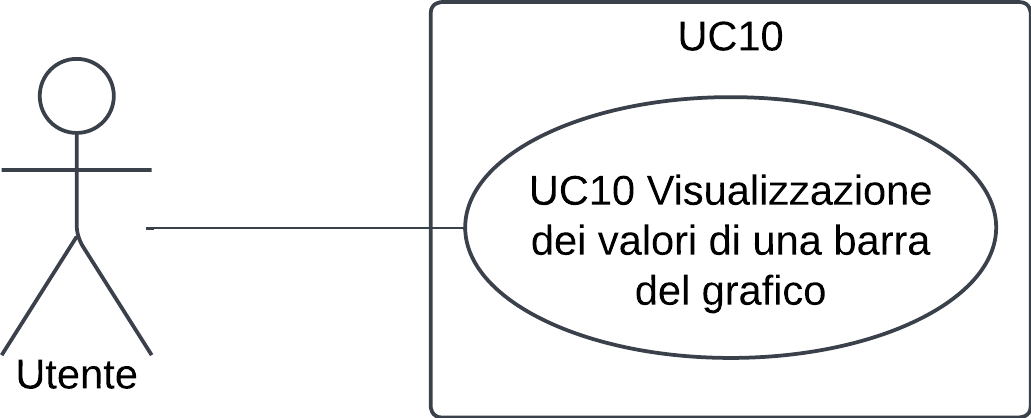
\includegraphics[scale=0.7]{template/images/UC10.png}
    \caption{UC10 - Visualizzare i valori di una barra del grafico}
\end{figure}
\begin{itemize}    
    \item \textbf{Attore:} utente;
    \item \textbf{Descrizione:} L'utente, tramite interazione opportuna, può selezionare una barra del grafico all'interno dell'ambiente 3D per visualizzarne i rispettivi valori.
    \item \textbf{Precondizioni:}    
        \begin{itemize}
            \item Il caricamento del dataset è avvenuto con successo.
            \item La generazione dell'ambiente 3D e del relativo grafico non hanno riscontrato errori.
            \item Viene eseguita l'interazione opportuna da parte dell'utente per la selezione della barra del grafico.
        \end{itemize}    
    \item \textbf{Postcondizioni:}
        \begin{itemize}
            \item Vengono visualizzati a schermo i valori della barra del grafico selezionata.
        \end{itemize}    
    \item \textbf{Scenario:} 
        \begin{itemize}
            \item L'utente interagisce con l'ambiente 3D e seleziona una barra del grafico per far apparire a schermo i valori.
        \end{itemize}
\end{itemize}

\subsection{UC11: Selezione elementi}
\begin{figure}[h!]\centering
    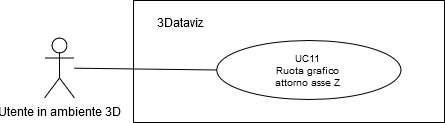
\includegraphics[scale=0.7]{template/images/UC11.png}
    \caption{UC11: Selezione elementi}
\end{figure}
\begin{itemize}    
    \item \textbf{Attore:} utente;
    \item \textbf{Descrizione:} L'utente, tramite interazione opportuna, può selezionare una barra del grafico all'interno dell'ambiente 3D oppure una singola cella nella tabella.
    \item \textbf{Precondizioni:}    
        \begin{itemize}
            \item Il caricamento del dataset è avvenuto con successo.
            \item La generazione dell'ambiente 3D e del relativo grafico non hanno riscontrato errori.
            \item La generazione della tabella non ha riscontrato errori.
            \item Viene eseguita l'interazione opportuna da parte dell'utente per la selezione.
        \end{itemize}    
    \item \textbf{Postcondizioni:}
        \begin{itemize}
            \item Viene evidenziata la selezione.
        \end{itemize}    
    \item \textbf{Scenario:} 
        \begin{itemize}
            \item L'utente interagisce con l'ambiente 3D e seleziona una barra del grafico oppure seleziona una cella della tabella.
        \end{itemize}
\end{itemize}

\pagebreak

\subsubsection{UC11.1: Selezione di un elemento del grafico}
\begin{figure}[h!]\centering
    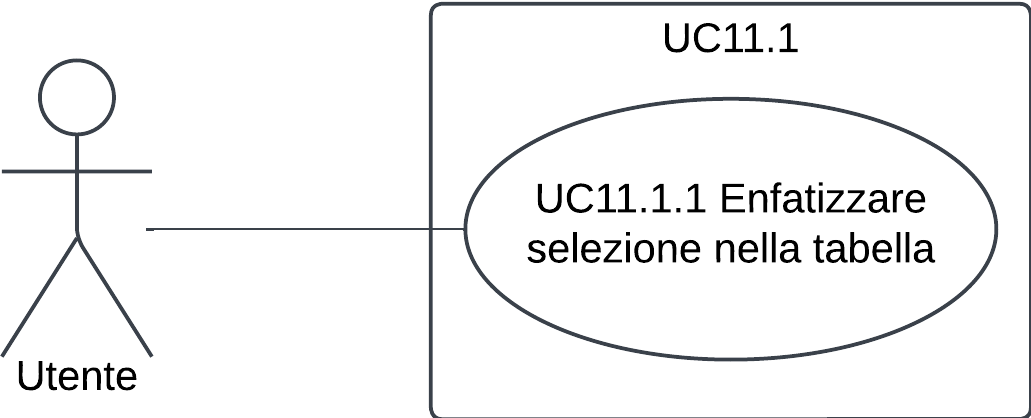
\includegraphics[scale=0.7]{template/images/UC11.1.png}
    \caption{UC11.1: Selezione di un elemento del grafico}
\end{figure}
\begin{itemize}    
    \item \textbf{Attore:} utente;
    \item \textbf{Descrizione:} L'utente, tramite interazione opportuna, può selezionare una barra del grafico all'interno dell'ambiente 3D.
    \item \textbf{Precondizioni:}    
        \begin{itemize}
            \item Il caricamento del dataset è avvenuto con successo.
            \item La generazione dell'ambiente 3D e del relativo grafico non hanno riscontrato errori.
            \item Viene eseguita l'interazione opportuna da parte dell'utente per la selezione.
        \end{itemize}    
    \item \textbf{Postcondizioni:}
        \begin{itemize}
            \item Viene evidenziata la selezione sia della barra del grafico selezionata sia della corrispetiva cella della tabella.
        \end{itemize}    
    \item \textbf{Scenario:} 
        \begin{itemize}
            \item L'utente interagisce con l'ambiente 3D e seleziona una barra del grafico.
        \end{itemize}
\end{itemize}
\paragraph{UC11.1.1: Enfatizzare selezione nella tabella}
\begin{itemize}    
    \item \textbf{Attore:} utente;
    \item \textbf{Descrizione:} Viene evidenziata in maniera opportuna nella tabella la selezione compiuta dall'utente.
    \item \textbf{Precondizioni:}    
        \begin{itemize}
            \item Il caricamento del dataset è avvenuto con successo.
            \item La generazione della tabella non ha riscontrato errori.
            \item Viene eseguita l'interazione opportuna da parte dell'utente per la selezione.
        \end{itemize}    
    \item \textbf{Postcondizioni:}
        \begin{itemize}
            \item Viene evidenziata la selezione nella tabella.
        \end{itemize}    
    \item \textbf{Scenario:} 
        \begin{itemize}
            \item L'utente interagisce con l'interfaccia e compie un'azione di selezione che viene evidenziata nella tabella.
        \end{itemize}
\end{itemize}

\pagebreak

\subsubsection{UC11.2: Selezione di una cella della tabella}
\begin{figure}[h!]\centering
    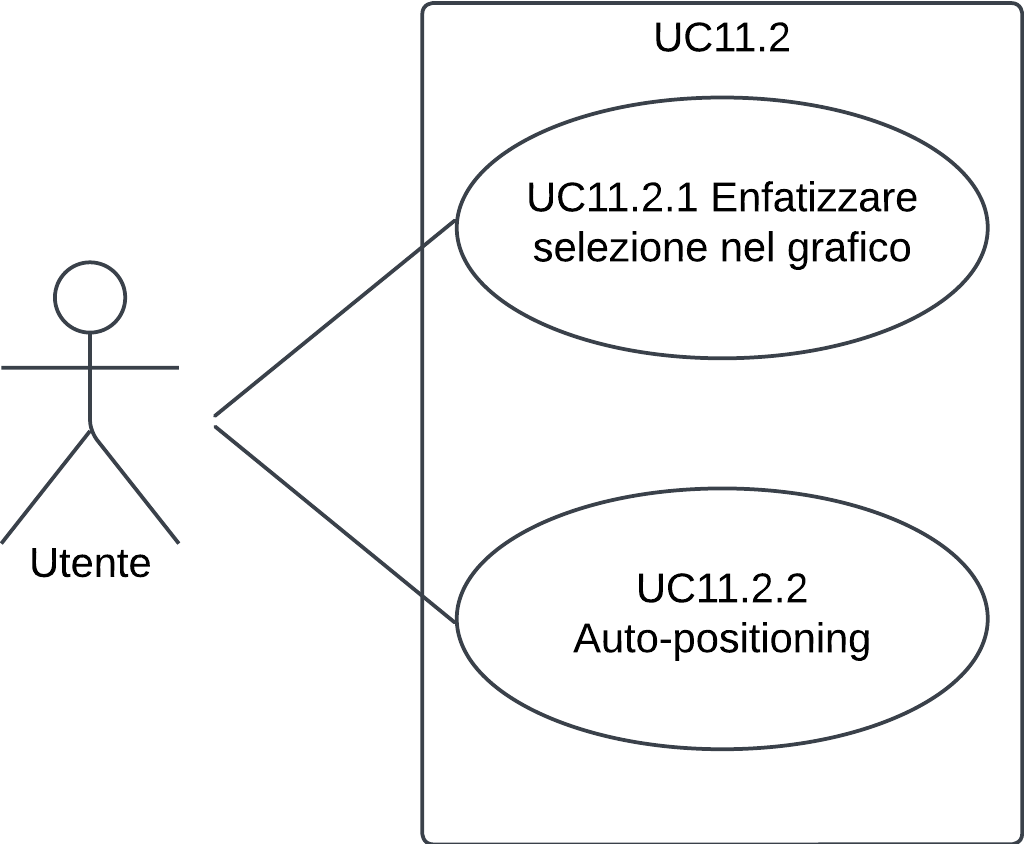
\includegraphics[scale=0.7]{template/images/UC11.2.png}
    \caption{UC11.2: Selezione di una cella della tabella}
\end{figure}
\begin{itemize}    
    \item \textbf{Attore:} utente;
    \item \textbf{Descrizione:} L'utente, tramite interazione opportuna, può selezionare una cella all'interno della tabella.
    \item \textbf{Precondizioni:}    
        \begin{itemize}
            \item Il caricamento del dataset è avvenuto con successo.
            \item La generazione della tabella non ha riscontrato errori.
            \item Viene eseguita l'interazione opportuna da parte dell'utente per la selezione della cella.
        \end{itemize}    
    \item \textbf{Postcondizioni:}
        \begin{itemize}
            \item Viene evidenziata la selezione sia della cella della tabella selezionata sia della corrispetiva barra del grafico all'interno dell'ambiente 3D.
        \end{itemize}    
    \item \textbf{Scenario:} 
        \begin{itemize}
            \item L'utente interagisce con la tabella selezionando una cella.
        \end{itemize}
\end{itemize}
\paragraph{UC11.2.1: Enfatizzare selezione nel grafico}
\begin{itemize}    
    \item \textbf{Attore:} utente;
    \item \textbf{Descrizione:} Viene evidenziata in maniera opportuna nel grafico all'interno dell'ambiente 3D la selezione compiuta dall'utente.
    \item \textbf{Precondizioni:}    
        \begin{itemize}
            \item Il caricamento del dataset è avvenuto con successo.
            \item La generazione dell'ambiente 3D e del relativo grafico non hanno riscontrato errori.
            \item Viene eseguita l'interazione opportuna da parte dell'utente per la selezione.
        \end{itemize}    
    \item \textbf{Postcondizioni:}
        \begin{itemize}
            \item Viene evidenziata la selezione nel grafico all'interno dell'ambiente 3D.
        \end{itemize}    
    \item \textbf{Scenario:} 
        \begin{itemize}
            \item L'utente interagisce con l'interfaccia e compie un'azione di selezione che viene evidenziata nel grafico all'interno dell'ambiente 3D.
        \end{itemize}
\end{itemize}
\paragraph{UC11.2.2: Auto-positioning}
\begin{itemize}    
    \item \textbf{Attore:} utente;
    \item \textbf{Descrizione:} La posizione della telecamera e l'inquadratura vengono posizinate in maniera consona in modo tale da ottenere in primo piano uno specifico oggetto all'interno dell'ambiente 3D.
    \item \textbf{Precondizioni:}    
        \begin{itemize}
            \item Il caricamento del dataset è avvenuto con successo.
            \item La generazione dell'ambiente 3D e del relativo grafico non hanno riscontrato errori.
            \item Viene richiesta un'operazione di auto-positioning.
        \end{itemize}    
    \item \textbf{Postcondizioni:}
        \begin{itemize}
            \item La telecamera e la relativa inquadratura saranno in una posizione diversa da quella iniziale e avranno inoltre in primo piano uno specifico oggetto dell'ambiente 3D.
        \end{itemize}    
    \item \textbf{Scenario:} 
        \begin{itemize}
            \item L'utente seleziona una cella della tabella e la telecamera nell'ambiente 3D si sposta di conseguenza inquadrando la corrispettiva barra del grafico.
        \end{itemize}
\end{itemize}

\subsection{UC12: Opacizzare barra del grafico}
\begin{figure}[h!]\centering
    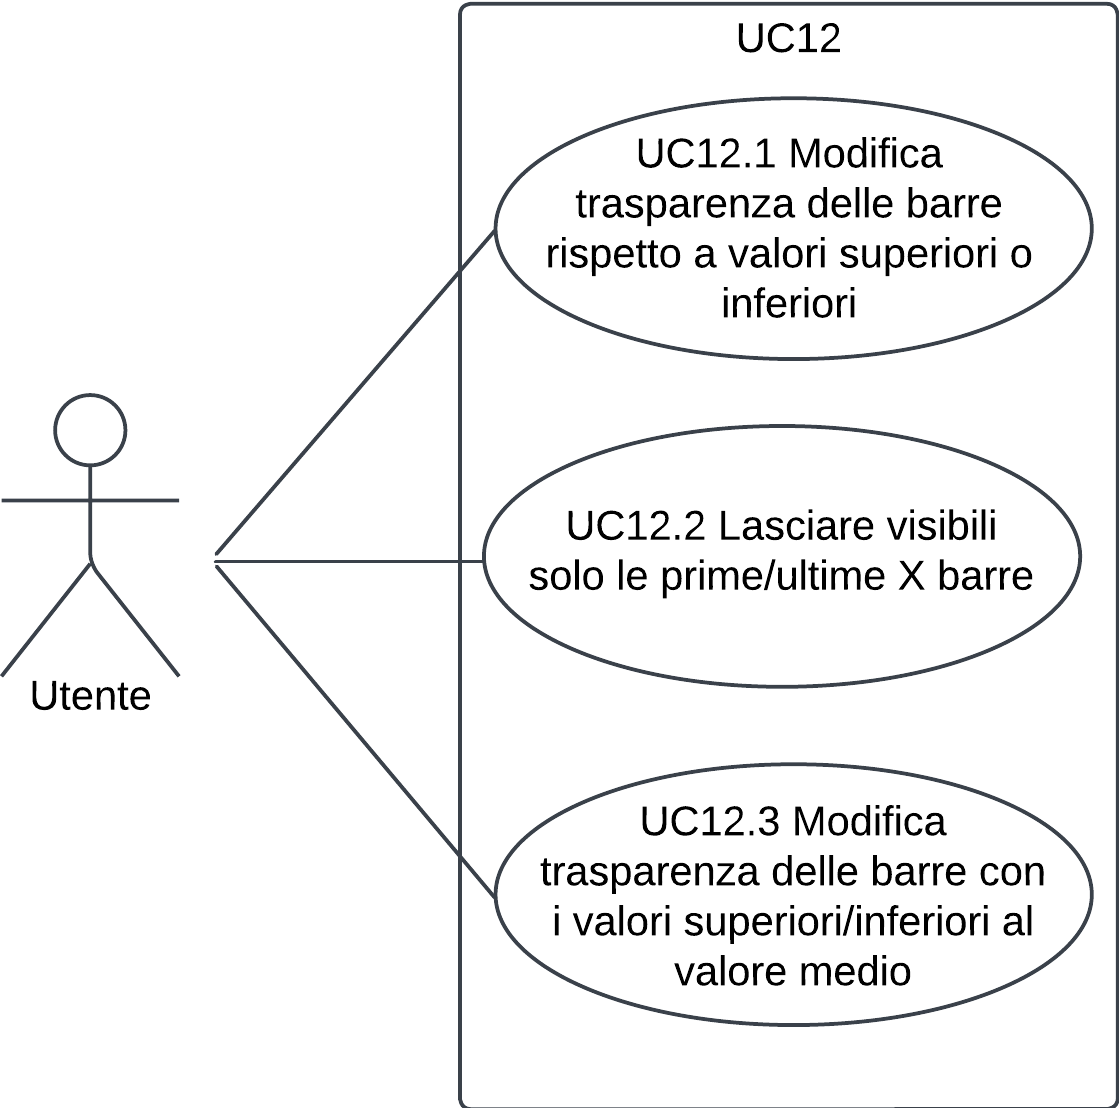
\includegraphics[scale=0.7]{template/images/UC12.png}
    \caption{UC12: Opacizzare barra del grafico}
\end{figure}
\begin{itemize}    
    \item \textbf{Attore:} utente;
    \item \textbf{Descrizione:} Viene aumentata la trasparenza di una barra del grafico all'interno dell'ambiente 3D.
    \item \textbf{Precondizioni:}    
        \begin{itemize}
            \item Il caricamento del dataset è avvenuto con successo.
            \item La generazione dell'ambiente 3D e del relativo grafico non hanno riscontrato errori.
        \end{itemize}    
    \item \textbf{Postcondizioni:}
        \begin{itemize}
            \item Il valore di opacità di una barra del grafico nell'ambiente 3D è maggiore rispetto al valore iniziale.
        \end{itemize}    
    \item \textbf{Scenario:} 
        \begin{itemize}
            \item Per evidenziare una determinata barra del grafico vengono opacizzate tutte le altre.
        \end{itemize}
\end{itemize}
\subsubsection{UC12.1: Opacizzare le barre rispetto a valori superiori o inferiori}
\begin{itemize}    
    \item \textbf{Attore:} utente;
    \item \textbf{Descrizione:} L'utente interagisce opportunamente con l'interfaccia impostando un valore rispetto al quale ogni barra con valore superiore o inferiore (parametro specificato dall'utente) verrà opacizzata.
    \item \textbf{Precondizioni:}    
        \begin{itemize}
            \item Il caricamento del dataset è avvenuto con successo.
            \item La generazione dell'ambiente 3D e del relativo grafico non hanno riscontrato errori.
            \item La generazione dell'interfaccia non ha riscontrato errori
            \item L'utente imposta correttamente tutti i parametri necessari.
        \end{itemize}    
    \item \textbf{Postcondizioni:}
        \begin{itemize}
            \item Ogni barra con il rispettivo valore che non rispetta le condizioni poste dall'utente verrà opacizzata.
        \end{itemize}    
    \item \textbf{Scenario:} 
        \begin{itemize}
            \item L'utente interagisce con l'interfaccia per evidenziare nel grafico all'interno dell'ambiente 3D solo le barre con un valore superiore/inferiore a quello indicato.
        \end{itemize}
\end{itemize}
\subsubsection{UC12.2: Lasciare visibili solo le prime/ultime X barre}
\begin{itemize}    
    \item \textbf{Attore:} utente;
    \item \textbf{Descrizione:} L'utente può evidenziare le X barre più piccole/grandi.
    \item \textbf{Precondizioni:}    
        \begin{itemize}
            \item Il caricamento del dataset è avvenuto con successo.
            \item La generazione dell'ambiente 3D e del relativo grafico non hanno riscontrato errori.
            \item La generazione dell'interfaccia non ha riscontrato errori
            \item L'utente imposta correttamente tutti i parametri necessari.
        \end{itemize}    
    \item \textbf{Postcondizioni:}
        \begin{itemize}
            \item Ogni barra del grafico nell'ambiente 3D con il rispettivo valore che non rientra nei primi X valori più piccoli/grandi viene opacizzata.
        \end{itemize}    
    \item \textbf{Scenario:} 
        \begin{itemize}
            \item L'utente interagisce con l'interfaccia per evidenziare nel grafico all'interno dell'ambiente 3D le prime X barre con il corrispettivo valore che rientra nei primi X valori più piccoli/grandi.
        \end{itemize}
\end{itemize}